\documentclass[10pt]{article}

%==============================================================================
% PREAMBLE — styled after the AutoAgent technical-report format (matching the
% GAUSE explainer): blue numbered headings, rounded boxed abstract, dotted ToC
% leaders, "Figure N" captions, and full-width illustrative diagrams.
%==============================================================================
\usepackage[margin=1in]{geometry}
\usepackage{amsmath, amssymb, amsthm}
\usepackage{booktabs}
\usepackage{graphicx}
\usepackage{enumitem}
\usepackage{xcolor}
\usepackage{tikz}
\usetikzlibrary{positioning, arrows.meta, calc, shapes.misc, backgrounds, fit}
\usepackage{pgfplots}
\pgfplotsset{compat=1.18}
\usepackage[most]{tcolorbox}
\tcbuselibrary{skins}
\usepackage{titlesec}
\usepackage{tocloft}
\usepackage[labelfont=bf, labelsep=quad, font=small]{caption}

% --- Color palette (AutoAgent-style) ---
\definecolor{headblue}{RGB}{61, 107, 191}     % section headings, links
\definecolor{absbg}{RGB}{235, 242, 252}       % abstract box background
\definecolor{popblue}{RGB}{222, 235, 250}     % RISP panel fill
\definecolor{popblueD}{RGB}{90, 130, 200}     % RISP panel frame
\definecolor{reworange}{RGB}{253, 238, 222}   % reward-driven panel fill
\definecolor{reworangeD}{RGB}{226, 140, 60}   % reward-driven panel frame
\definecolor{okgreen}{RGB}{60, 145, 90}
\definecolor{badred}{RGB}{200, 60, 60}
\definecolor{dormgray}{RGB}{150, 150, 150}

\usepackage[colorlinks=true, linkcolor=headblue, citecolor=headblue,
            urlcolor=headblue]{hyperref}

% --- Blue numbered headings ---
\titleformat{\section}{\Large\bfseries\color{headblue}}{\thesection}{0.8em}{}
\titleformat{\subsection}{\large\bfseries\color{headblue}}{\thesubsection}{0.8em}{}
\titleformat{\subsubsection}{\normalsize\bfseries\color{headblue}}{\thesubsubsection}{0.8em}{}

% --- Dotted leaders in the table of contents ---
\renewcommand{\cftsecleader}{\cftdotfill{\cftdotsep}}
\renewcommand{\cftsecfont}{\normalsize}
\renewcommand{\cftsecpagefont}{\normalsize}
\setcounter{tocdepth}{2}

% --- Boxed abstract (rounded, light blue) ---
\newtcolorbox{abstractbox}{enhanced, breakable, colback=absbg, colframe=headblue!45,
  boxrule=0.6pt, arc=8pt, left=14pt, right=14pt, top=8pt, bottom=10pt}

% --- Design/recipe callout box ---
\newtcolorbox{designbox}{colback=blue!4, colframe=headblue!55, boxrule=0.5pt,
  arc=3pt, left=8pt, right=8pt, top=5pt, bottom=5pt}

\newtheorem{observation}{Observation}
\newtheorem{principle}{Principle}
\newtheorem{proposition}{Proposition}

\newcommand{\E}{\mathbb{E}}
\newcommand{\Var}{\mathrm{Var}}
\newcommand{\nm}{\textsc{RISP}}

% --- TikZ styles shared by the diagrams ---
\tikzset{
  panel/.style={rounded corners=4pt, draw=#1, thick, inner sep=8pt},
  blk/.style={rounded corners=2.5pt, draw=#1!70!black, fill=#1!18, thick,
              align=center, font=\footnotesize, inner sep=4pt},
  chip/.style={rounded corners=2pt, draw=#1!70!black, fill=#1!25,
               align=center, font=\scriptsize, inner sep=3pt,
               minimum width=1.35cm, minimum height=0.5cm},
  lay/.style={rounded corners=2pt, draw=#1!75!black, fill=#1!15,
              align=center, font=\scriptsize, inner sep=2.5pt,
              minimum width=3.1cm, minimum height=0.52cm},
  arr/.style={-{Stealth[length=2.4mm]}, thick},
  lbl/.style={font=\scriptsize, align=center},
}

\title{\textbf{\nm{}: Retention and Invariance in Decision-Focused\\
Strategy Pools for Non-Stationary Markets}\\[0.35cm]
\large An Explanatory Companion: Architecture, Mechanisms, Demonstrations,
and Applications}

\author{Yuhao Li\thanks{Contact: Yuhao Li (\texttt{li88@sas.upenn.edu}).}\\
University of Pennsylvania}

\date{June 2026}

\begin{document}

\maketitle

\begin{abstractbox}
\begin{center}
{\color{headblue}\large\bfseries Abstract}
\end{center}
\noindent
Trading systems that must serve many market regimes with capacity-limited
strategy specialists face two allocation problems that are usually conflated
into one. The first is \emph{between regimes}: market states recur on
irregular schedules with long dormancy, and any mechanism that allocates
capital, attention, or recalibration by chasing current reward---a trailing-%
Sharpe capital allocator, a learned mixture-of-experts gate---systematically
starves and overwrites the specialist for whichever regime is dormant,
then pays a full relearning cost in the very window where decisions matter
most: the first days after the regime returns. The second is \emph{within} a
regime: each recurrence is a distinct draw from the regime's environment
distribution---the 2008 crisis is not 2020 is not 2022---so even a perfectly
retained specialist fails out-of-distribution on the next episode if it was
trained by empirical risk minimization on the last one. To address both, we
present \textbf{\nm{}} (Regime-Invariant Specialist Pools), a population-learning framework
for decision-focused (predict-then-optimize) trading built from three
tightly coupled components: \emph{per-regime decision heads} (linear SPO+
predictors feeding an exact portfolio optimizer, scored by decision regret
rather than prediction error), \emph{niche-affinity tracking} (the canonical
exponentiated-gradient update on the regime simplex, driven by batched
winner-take-all competition), and \emph{episode-invariant niche training}
(each specialist minimizes the variance plus mean of its regret surrogate
across the historical episodes of its own regime). The converged
regime-to-specialist assignment is \emph{reward-independent}---a crisis
specialist holds its niche by identity and idles through calm markets,
retaining both its parameters and its episode memory---while the invariance
objective makes what is retained \emph{general} across episodes rather than
calibrated to the last one. We prove a post-reactivation regret bound that
splits into a forgetting deficit (zero for any reward-independent covering
assignment; tending to the full relearning cost for any reward-chasing one)
and an invariance gap (controlled by the episode-variance penalty, with a
one-step Pinsker bridge from divergence-style invariance guarantees to
regret). In controlled regime-switching markets at realistic signal-to-noise,
every pre-registered prediction of the resulting $2{\times}2$ holds (20
seeds, Holm-corrected): the retention axis is worth $6.1\%$ of
post-reactivation regret ($p{=}1.3{\times}10^{-3}$), the invariance axis a
further $4.4\%$ ($p{=}6.1{\times}10^{-3}$), jointly $10.3\%$
($p{=}9.2{\times}10^{-7}$; $38\%$ of the excess above the irreducible noise
floor)---and the interaction is \emph{super-additive}: the invariance
objective is statistically inert inside a reward-driven monolith
($p{=}0.88$), because no training objective can help a head that was evicted
during dormancy. The full system is statistically indistinguishable from a
hand-pinned oracle assignment trained with the same objective ($p{=}0.72$):
competition recovers the skyline it was never shown. We are equally explicit
about what did \emph{not} work: a pre-registered structure diagnostic on real
crypto and commodity panels finds \emph{no exploitable regime structure on
the decision metric} under causal labelings, the real-data dissociation is
therefore correctly null, our batching expectation for the competition
window was refuted by the ablation, and the mechanism's advantage
\emph{inverts} (up to $-49\%$) when within-regime signal becomes strong
enough to chase---a measured crossover, not a caveat. We close with an
evidence-tiered application survey: multi-strategy capital allocation and
risk-model committees (mechanism-level evidence), and the conditions under
which one should \emph{not} deploy the framework. Code and per-figure result
files are released with the companion paper.
\end{abstractbox}

\vspace{0.25cm}
\noindent\textbf{Keywords:} regime switching; decision-focused learning;
catastrophic forgetting; invariant risk; strategy pools; reward-independent
assignment; competitive exclusion

\newpage
\tableofcontents
\newpage

%==============================================================================
\section{Introduction}
%==============================================================================

\begin{center}
\itshape``The time to repair the roof is when the sun is shining.''\\[2pt]
\normalfont ---J.~F.~Kennedy, on a different allocation problem
\end{center}

Every multi-strategy trading operation maintains expertise it is not
currently using. The crisis playbook idles through years of calm. The
short-volatility book hibernates through stress. The breakout system waits
out the range. This standing inventory of dormant competence is expensive
---infrastructure, attention, calibration---and so every such operation
also runs an allocator that decides, day by day, which strategies receive
capital and which receive maintenance. The allocator that practice and
machine learning both reach for first is \emph{reward-chasing}: trailing
performance weights, a learned gate, a router trained on realized P\&L.

The GAUSE study \cite{li2026gause} isolated, in controlled prediction
domains, why that default quietly destroys the inventory it is supposed to
manage: \textbf{a dormant regime emits no reward}. Whatever signal the
allocator uses to protect capacity is exactly the signal a dormant regime
does not produce, so reward-driven allocation reallocates the dormant
specialist's capacity to active regimes---hard eviction or gradual
interference, the result is the same---and the system relearns its crisis
playbook \emph{during the crisis}. GAUSE's resolution was structural:
winner-take-all competition over niches converges to an assignment that is
\emph{independent of current reward}, so dormant specialists idle and
retain, with no freezing schedule and no gate to train.

This companion document explains \nm{}, which ports that mechanism to
decision-focused financial learning and discovers, in doing so, that
retention is only \emph{half} of the financial problem. The other half has
no analogue in GAUSE's setting and comes from the invariant-learning
literature \cite{arjovsky2019irm, peters2016causal, yan2026invpnco}:
\textbf{regimes do not return unchanged}. A retained crisis specialist
knows the \emph{last} crisis---its correlations, its liquidity pattern,
its episode-specific accidents. If it was trained by empirical risk
minimization (ERM), it has loaded on those accidents (they were
predictive, in-sample), and the next crisis, a fresh draw from the crisis
distribution, punishes exactly that loading. Protecting the specialist's
memory protects the overfitting too. What must be retained is not the
calibration to the last episode but the \emph{decision-relevant structure
common to all episodes}---and that is a property of the training
objective, not of the allocator.

\nm{} therefore couples two mechanisms, each useless without the other:

\begin{enumerate}[leftmargin=1.8em]
    \item \textbf{Reward-independent capacity assignment} (solves
    between-regime forgetting). Specialists acquire regimes through
    batched winner-take-all competition; an exponentiated-gradient
    affinity update converges to a one-per-regime covering assignment
    which is then pinned. The crisis specialist holds its niche by
    identity. During dormancy it receives \emph{zero} foreign updates:
    its decision heads and its stored episode library are structurally
    untouchable.
    \item \textbf{Episode-invariant niche training} (solves within-regime
    drift). Each specialist trains its niche's decision head on the
    variance \emph{plus} mean of an SPO-style regret surrogate across
    the stored episodes of its own regime. Loading on episode-specific
    regularities inflates the across-episode variance and is penalized
    away; what survives is the structure every episode shares---which is
    precisely what the \emph{next} episode will reward.
\end{enumerate}

The framework's headline empirical object is a $2{\times}2$: allocation
mechanism (reward-driven vs.\ reward-independent) crossed with training
objective (ERM vs.\ invariant), evaluated by \emph{post-reactivation
decision regret}---mean regret in the first fifteen trading days after a
dormant regime returns. The companion paper's experiments confirm monotone
improvement along both axes \emph{and} the signature interaction that
makes the two-mechanism account falsifiable: the invariance objective does
\textbf{nothing} inside a reward-driven monolith ($p = 0.88$ against ERM),
because the head it trained was evicted during dormancy; it pays only
inside a retaining allocation ($-4.4\%$, $p = 6.1 \times 10^{-3}$). Each
mechanism is the other's precondition.

This document is the explanatory companion to the research paper. It
develops the architecture component by component
(Section~\ref{sec:framework}), walks through the two non-stationarities
with worked numerical demonstrations (Sections~\ref{sec:decision}--%
\ref{sec:competition}), states the reward-independence principle and the
regret decomposition at an accessible level of rigor
(Section~\ref{sec:principle}), surveys the experimental evidence
including every result that came out against us
(Section~\ref{sec:experiments}), and maps the application terrain with
explicit evidence tiers and an honest ``when not to use it''
(Section~\ref{sec:applications}).

\paragraph{Reading guide.} Readers wanting the mechanism:
Sections~\ref{sec:framework}--\ref{sec:competition}. Readers wanting the
theory: Section~\ref{sec:principle} here, full proofs in the mathematical
deep-dive companion. Readers evaluating deployment:
Sections~\ref{sec:experiments} and \ref{sec:applications}, especially
\ref{sec:whennot}. Readers auditing our honesty: every subsection labeled
``what did not survive.''

%==============================================================================
\section{Related Work}
%==============================================================================

We position \nm{} along five lines, ordered by proximity.

\textbf{GAUSE and reward-independent specialization.} GAUSE
\cite{li2026gause} established, across six real prediction domains and
controlled non-stationarity protocols, that retention of dormant regimes
under bounded capacity tracks a single property---reward-independence of
the capacity assignment plus persistent coverage---and that winner-take-all
competition reaches that assignment emergently, matching an oracle fixed
assignment without being given it. \nm{} is the decision-focused,
financial instantiation: quality is decision regret rather than prediction
reward, competition is batched into multi-day windows, and---the new
axis---retained specialists are trained for episode invariance. Everything
GAUSE proved about its own scope (the SI-organization audit, the
task-incremental framing, the stale-specialist liability under drift) is
inherited and re-audited here in the decision setting.

\textbf{Decision-focused learning.} The smart predict-then-optimize
framework \cite{elmachtoub2022smart}, its surrogates for hard
combinatorial layers \cite{mandi2020smart, shah2022lodl}, and the field
survey \cite{mandi2024decision} establish why decision regret, not
prediction error, is the right training and evaluation signal when
forecasts feed an optimizer. All assume stationarity or one-shot shift.
Inv-PnCO \cite{yan2026invpnco} adds invariant learning across environments
for predict-and-optimize, bounding divergences between solution
distributions. We adapt its environment-indexed objective to
\emph{recurring} regimes (episodes as environments) and add the
allocation axis it has no occasion to consider; our Pinsker-type lemma
converts its divergence-style guarantees into the regret currency our
bound is stated in.

\textbf{Regime-switching finance.} From Markov-switching models
\cite{hamilton1989new} through regime-aware allocation
\cite{ang2012regime, guidolin2007asset, nystrup2018dynamic,
nystrup2020greedy}, this literature detects regimes and conditions a
single model. Conditioning answers ``what is true now''; it does not
answer ``who keeps what is true about \emph{then}.'' Our capacity-bounded
regime-conditioned monolith is this literature's best case under a memory
budget, and the dissociation experiments measure precisely what
conditioning alone forfeits.

\textbf{Online learning over experts.} Hedge and multiplicative weights
\cite{freund1997decision, arora2012multiplicative}, universal portfolios
\cite{cover1991universal, li2014online}, and sleeping experts / adaptive
regret \cite{freund1997sleeping, hazan2009adaptive, daniely2015strongly}
are the closest formal relatives and the most dangerous deflation: ``is
this not just sleeping experts?'' No---and the difference is load-bearing.
Sleeping-experts theory combines \emph{fixed} experts, which retain
dormant state because there is nothing in them to forget. When experts are
capacity-bounded \emph{learners}, the combination weights are
reward-driven and training resources follow the weights, which
reintroduces interference. We run both readings as baselines: Hedge over
fixed strategies retains and loses everywhere (it cannot adapt
within-regime); Hedge over learning experts adapts and forgets (it tracks
the monolith). The contribution lives in the bracket between them.

\textbf{Continual learning.} Catastrophic forgetting
\cite{french1999catastrophic, parisi2019continual} and its single-model
remedies (EWC \cite{kirkpatrick2017overcoming}, progressive networks
\cite{rusu2016progressive}) treat retention as a regularization or
architecture problem. MoE continual-learning theory \cite{li2024moecl}
shows expert isolation mitigates forgetting provided the gate's updates
eventually stop---in our vocabulary, provided the assignment becomes
reward-independent. The population mechanism reaches that state with no
schedule; the financial contribution of this work is what must be
\emph{added} to retention (invariance) once the environment's recurrences
are themselves heterogeneous.

%==============================================================================
\section{The \nm{} Framework: Architecture for Two Non-Stationarities}
\label{sec:framework}
%==============================================================================

\subsection{Design Philosophy: Separate the Two Clocks}

Financial non-stationarity runs on two clocks. The \emph{fast clock} is
regime switching: every few weeks or months the market's character changes
---trend to range, calm to stressed---and the change is largely a
\emph{return} to a previously seen state. The \emph{slow clock} is
within-regime evolution: each return differs from the last, because the
market's microstructure, participants, and transmission channels drift
between occurrences. A system built only for the fast clock (retain every
regime's specialist) arrives at the next crisis perfectly calibrated to
the previous one. A system built only for the slow clock (one robust
invariant model) averages away the regime structure entirely. The design
philosophy of \nm{} is that the two clocks demand two separate mechanisms
coupled through one object---the \emph{specialist}:

\begin{designbox}
\textbf{The \nm{} recipe.} One specialist per regime, discovered by
competition, held by identity, trained for invariance:
\begin{enumerate}[leftmargin=1.6em, nosep]
    \item \emph{Compete}: all specialists shadow-trade every day; cumulative
    decision regret over a $W_c$-day window within the active regime
    selects a window winner.
    \item \emph{Specialize}: the winner reinforces its niche affinity for
    the active regime (exponentiated-gradient on the regime simplex) and
    trains on the window's data.
    \item \emph{Pin}: when an affinity crosses $0.95$, the regime is
    pinned to its owner; allocation stops responding to reward---the
    retention guarantee becomes structural.
    \item \emph{Generalize}: owners train their niche's decision head on
    $\Var_e[\text{regret surrogate}] + \beta\,\E_e[\text{regret
    surrogate}]$ across the stored episodes $e$ of their regime---never on
    one episode alone.
\end{enumerate}
\end{designbox}

Three deliberate omissions define the architecture as much as its
components. There is \textbf{no gate}: routing is by the converged
assignment, so there is no reward-trained module whose blindness to
dormant regimes could erode the inventory. There is \textbf{no freezing
schedule}: pinning is triggered by the affinity dynamics themselves, not
by a hand-set epoch. And there is \textbf{no hand-designed regime-to-desk
map}: the assignment is discovered, which matters less because design is
hard (a fund can silo desks by hand) than because the discovered
assignment provably matches the hand-designed skyline while degrading
gracefully when the regime inventory is misjudged.

\subsection{Architectural Blueprint}

Figure~\ref{fig:architecture} shows the data path. Each trading day, a
causal labeler maps public information through $t-1$ to a regime label
$r_t$ (volatility band $\times$ trend sign in the headline configuration;
a filtered two-state model as the robustness alternative). Each
specialist $i$ holds: a \emph{niche affinity} $\alpha_i \in \Delta^R$
(its identity---where it belongs); up to $K$ \emph{decision heads}
$w_{i,r} \in \mathbb{R}^d$ (its competence---linear SPO+ predictors per
held regime); and a bounded \emph{episode library} per held regime (its
memory---the raw material for the invariance objective). The serving path
is regime label $\to$ owner $\to$ head $\to$ predicted returns $\to$
exact portfolio optimizer $\to$ decision. The learning path adds: regret
of every specialist's shadow decision $\to$ window accumulator $\to$
winner $\to$ EG affinity update + invariant training step.

\begin{figure}[t]
\centering
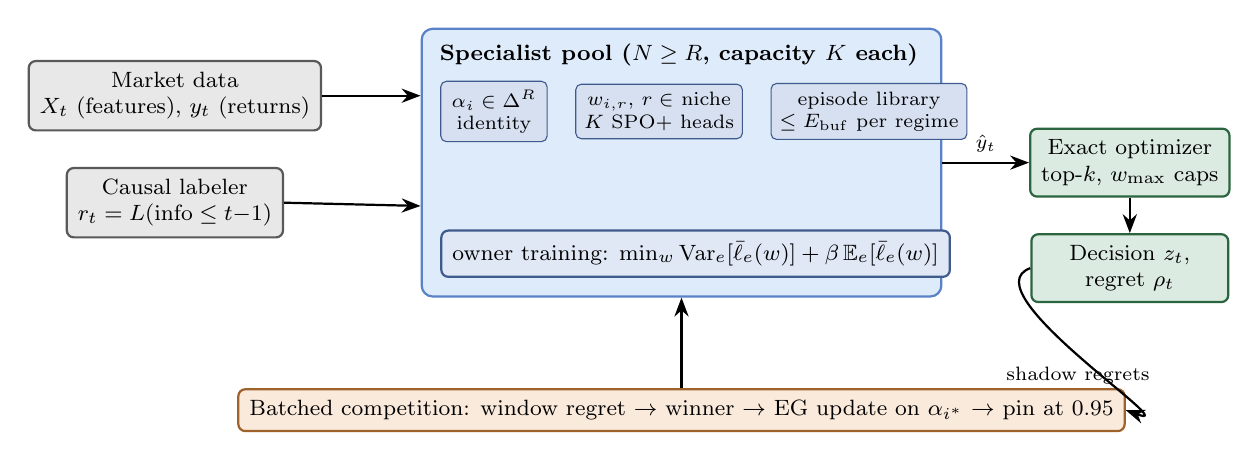
\begin{tikzpicture}[node distance=0.55cm and 0.7cm]
  % Market data input
  \node[blk=gray, minimum width=2.6cm] (mkt) {Market data\\ $X_t$ (features), $y_t$ (returns)};
  \node[blk=gray, minimum width=2.6cm, below=0.45cm of mkt] (lab)
    {Causal labeler\\ $r_t = L(\text{info} \le t{-}1)$};
  % Specialist panel
  \node[panel=popblueD, fill=popblue, minimum width=6.6cm, minimum height=3.4cm,
        right=1.25cm of mkt, yshift=-0.85cm] (pop) {};
  \node[font=\footnotesize\bfseries, anchor=north west] at ($(pop.north west)+(0.12,-0.08)$)
    {Specialist pool ($N \ge R$, capacity $K$ each)};
  \node[chip=popblueD, anchor=west] (a1) at ($(pop.west)+(0.25,0.65)$)
    {$\alpha_i \in \Delta^R$\\ \scriptsize identity};
  \node[chip=popblueD, right=0.35cm of a1] (heads)
    {$w_{i,r}$, $r \in$ niche\\ \scriptsize $K$ SPO+ heads};
  \node[chip=popblueD, right=0.35cm of heads] (lib)
    {episode library\\ \scriptsize $\le E_{\mathrm{buf}}$ per regime};
  \node[blk=popblueD, anchor=south west, minimum width=5.9cm]
    (inv) at ($(pop.south west)+(0.25,0.25)$)
    {owner training: $\min_w \Var_e[\bar\ell_e(w)] + \beta\,\E_e[\bar\ell_e(w)]$};
  % Decision layer
  \node[blk=okgreen, right=1.1cm of pop, minimum width=2.5cm] (opt)
    {Exact optimizer\\ top-$k$, $w_{\max}$ caps};
  \node[blk=okgreen, below=0.45cm of opt, minimum width=2.5cm] (dec)
    {Decision $z_t$,\\ regret $\rho_t$};
  % Competition loop
  \node[blk=reworangeD, below=1.15cm of pop, minimum width=6.4cm] (comp)
    {Batched competition: window regret $\to$ winner $\to$ EG update on
    $\alpha_{i^*}$ $\to$ pin at $0.95$};
  % Arrows
  \draw[arr] (mkt.east) -- ($(pop.west)+(0,0.85)$);
  \draw[arr] (lab.east) -- ($(pop.west)+(0,-0.55)$);
  \draw[arr] (pop.east) -- node[lbl, above]{$\hat y_t$} (opt.west);
  \draw[arr] (opt) -- (dec);
  \draw[arr] (dec.west) to[out=200, in=-20] node[lbl, below]{shadow regrets} (comp.east);
  \draw[arr] (comp.north) -- ($(pop.south)+(0,0)$);
\end{tikzpicture}
\caption{\nm{} architecture. Serving path (top): label $\to$ owner's head
$\to$ exact decision. Learning path (bottom): every specialist's shadow
regret feeds the batched competition, whose winner---and only the
winner---updates identity and competence. After pinning, the competition
loop is bypassed for that regime and the owner trains alone: allocation
has become reward-independent.}
\label{fig:architecture}
\end{figure}

\subsection{One Step of the Loop}

Concretely, a day in the converged system: the labeler reports
\texttt{vol-down} (the crisis-type regime). The pinned owner, specialist
3, loads its \texttt{vol-down} head---untouched for 280 days but neither
evicted nor decayed, because specialist 3 has won nothing and been
assigned nothing since its regime went dormant---and its episode library
holding the previous four \texttt{vol-down} episodes. It predicts
cross-sectional returns, the optimizer selects the top-$k$ caps-respecting
portfolio, and the realized regret is recorded. The owner then takes one
training step---\emph{not} on today's data alone, but on the variance-plus-
mean objective across its stored episodes including the new one: today's
data enters as the newest episode, and the objective immediately punishes
any weight that helps today's episode at the expense of the stored ones.
Meanwhile specialists 0--2 served and trained their own active or recent
niches; nobody touched specialist 3's other slots. Tomorrow, if the regime
persists, the same; if it ends, specialist 3 goes back to idling---with a
library now one episode richer.

%==============================================================================
\section{Decision-Focused Learning: Why Regret Is the Currency}
\label{sec:decision}
%==============================================================================

\subsection{The Predict-Then-Optimize Gap}

The decision layer is a cardinality-constrained long-only portfolio: pick
at most $k$ of $n$ assets at weight up to $w_{\max}$ to maximize
$y^\top z$. Because the objective is linear, the optimum is exact and
instantaneous (the $k$ largest positive predicted returns at full
weight), and the \emph{decision regret} of a forecast $\hat y$ against
realized $y$ is
\[
  \rho(\hat y; y) = \max_{z \in Z} y^\top z - y^\top z(\hat y) \ \ge 0 ,
\]
which is zero iff the forecast selects an optimal portfolio---regardless
of how wrong the forecast is numerically.

\begin{observation}[Prediction error is the wrong currency]
Two forecasts with identical mean-squared error can differ arbitrarily in
regret, and vice versa. A forecast that doubles every true return has
large MSE and \emph{zero} regret (rankings preserved); a forecast with
tiny MSE concentrated on swapping the $k$-th and $(k{+}1)$-th assets pays
regret on every such day. Training and evaluating specialists by
prediction error therefore optimizes---and audits---the wrong
object. \nm{} uses the SPO+ convex surrogate \cite{elmachtoub2022smart}
of $\rho$ for training (two oracle calls per gradient) and raw $\rho$ for
all evaluation and competition.
\end{observation}

This choice has an audit consequence worth flagging early: GAUSE's oracle
diagnostic found that crypto and commodity panels carry no exploitable
regime structure under \emph{prediction} metrics \cite{li2026gause}.
Since prediction-optimal and decision-optimal differ, that verdict does
not automatically transfer---structure invisible to MSE could in
principle matter for top-$k$ selection. Re-running the diagnostic under
the decision metric is therefore a genuine question, which our E0 answers
(Section~\ref{sec:exp-e0}): the null transfers. Honest, and not a
foregone conclusion.

\subsection{Worked Demonstration: When Retention Decides}

A miniature with $n = 4$ assets, $k = 1$, $w_{\max} = 1$. The crisis
regime's invariant structure says ``asset A (quality) outperforms; asset
D (leveraged) crashes,'' with true crisis-day returns
$y = (+2\%, 0\%, 0\%, -4\%)$.

\emph{Retained specialist} (held through 280 days of dormancy): predicts
$\hat y = (+1.5\%, +0.2\%, -0.1\%, -2.8\%)$---imperfect, but the ranking
is right. Decision: A. Regret $= 0$.

\emph{Relearning monolith} (evicted the crisis head during dormancy; two
days into refitting from prior): predicts noise around zero,
$\hat y = (+0.1\%, +0.4\%, +0.3\%, +0.2\%)$. Decision: B. Regret
$= 2\%$ of capital \emph{on that day}; integrated over a fifteen-day
probe window at crisis volatility, the relearning transient is the
dominant cost in the entire evaluation---which is exactly what the
companion paper's reactivation-aligned traces show at full scale
(monolith regret spikes $\sim 40\%$ above its steady state in the probe
window, while the retained owner is flat from day one).

\emph{Retained but episode-overfit specialist}: predicts from the
\emph{last} crisis's accident---say, in that episode, asset C's sector
happened to rally---$\hat y = (+1.2\%, 0\%, +1.8\%, -2.5\%)$. Decision:
C. Regret $= 2\%$. Retention preserved the head; ERM made the head worth
preserving less. This is the second axis, and no allocator fixes it.

%==============================================================================
\section{The Two Non-Stationarities, Visualized}
\label{sec:timeline}
%==============================================================================

Figure~\ref{fig:timeline} compresses the paper's thesis into one
timeline: a crisis regime that activates twice, with a long calm dormancy
between, drawn for the reward-driven monolith (top) and \nm{} (bottom).

\begin{figure}[t]
\centering
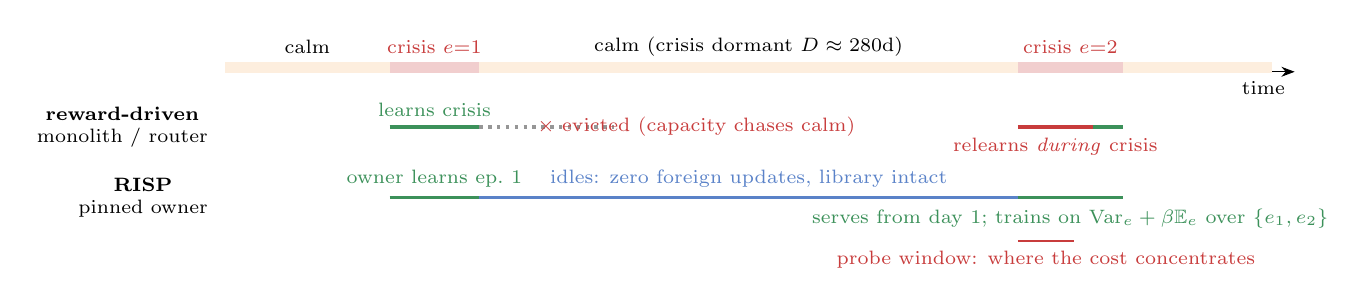
\begin{tikzpicture}[xscale=0.95]
  % time axis
  \draw[-{Stealth}] (0, 0) -- (14.3, 0) node[below left, font=\scriptsize]{time};
  % regime bands
  \fill[reworange] (0.0, -0.02) rectangle (2.2, 0.12);
  \fill[badred!25] (2.2, -0.02) rectangle (3.4, 0.12);
  \fill[reworange] (3.4, -0.02) rectangle (10.6, 0.12);
  \fill[badred!25] (10.6, -0.02) rectangle (12.0, 0.12);
  \fill[reworange] (12.0, -0.02) rectangle (14.0, 0.12);
  \node[lbl] at (1.1, 0.32) {calm};
  \node[lbl, text=badred] at (2.8, 0.32) {crisis $e{=}1$};
  \node[lbl] at (7.0, 0.32) {calm (crisis dormant $D \approx 280$d)};
  \node[lbl, text=badred] at (11.3, 0.32) {crisis $e{=}2$};
  % monolith lane
  \node[lbl, anchor=east] at (-0.1, -0.7) {\textbf{reward-driven}\\ monolith / router};
  \draw[very thick, okgreen] (2.2, -0.7) -- (3.4, -0.7)
    node[midway, above, lbl, text=okgreen]{learns crisis};
  \draw[very thick, dormgray, dotted] (3.4, -0.7) -- (5.2, -0.7);
  \node[lbl, text=badred] at (6.3, -0.7) {$\times$ evicted (capacity chases calm)};
  \draw[very thick, badred] (10.6, -0.7) -- (11.6, -0.7)
    node[midway, below, lbl, text=badred]{relearns \emph{during} crisis};
  \draw[very thick, okgreen] (11.6, -0.7) -- (12.0, -0.7);
  % risp lane
  \node[lbl, anchor=east] at (-0.1, -1.6) {\textbf{\nm{}}\\ pinned owner};
  \draw[very thick, okgreen] (2.2, -1.6) -- (3.4, -1.6)
    node[midway, above, lbl, text=okgreen]{owner learns ep.\ 1};
  \draw[very thick, popblueD] (3.4, -1.6) -- (10.6, -1.6)
    node[midway, above, lbl, text=popblueD]{idles: zero foreign updates, library intact};
  \draw[very thick, okgreen] (10.6, -1.6) -- (12.0, -1.6)
    node[midway, below, lbl, text=okgreen]{serves from day 1; trains on $\Var_e + \beta\E_e$ over $\{e_1, e_2\}$};
  % probe windows
  \draw[decorate, thick, badred] (10.6, -2.15) -- (11.35, -2.15)
    node[midway, below, lbl, text=badred]{probe window: where the cost concentrates};
\end{tikzpicture}
\caption{The two failure modes on one timeline. \textbf{Top lane:} a
reward-driven allocator learns the first crisis, evicts it during
dormancy (no reward $\Rightarrow$ no protection), and pays the relearning
transient inside the second crisis's probe window. \textbf{Bottom lane:}
the pinned owner idles through dormancy structurally untouched---and its
invariance objective across episodes $\{e_1, e_2, \dots\}$ keeps what it
retains general rather than calibrated to $e_1$'s accidents.}
\label{fig:timeline}
\end{figure}

The figure also locates the two ways to fail \emph{after} solving
retention, both measured in the companion paper's audits: if episodes are
heterogeneous and training is ERM, the bottom lane serves episode-1
calibration to episode 2 (the invariance axis, worth $4.4\%$ of probe
regret at baseline heterogeneity and growing with it); and if
within-regime signal is strong enough to refit in days, the top lane's
relearning transient shrinks until eviction stops mattering---at which
point chasing each episode \emph{beats} invariant retention (the E6
inversion, up to $-49\%$ at $8\times$ signal-to-noise). The mechanism has
boundaries, and both are drawn by experiment rather than assumption.

%==============================================================================
\section{Competition, Affinity, and Pinning}
\label{sec:competition}
%==============================================================================

\subsection{The Exponentiated-Gradient Affinity Update}

Each specialist's identity is a distribution $\alpha_i \in \Delta^R$ over
regimes, initialized uniform. When specialist $i^*$ wins a competition
window in regime $r$, it applies the canonical exponentiated-gradient
(Hedge / multiplicative-weights) update
\cite{kivinen1997exponentiated, freund1997decision,
arora2012multiplicative}:
\[
  \alpha_{i^*, r} \leftarrow \frac{\alpha_{i^*, r}\, e^{\eta}}
  {\sum_{q} \alpha_{i^*, q}\, e^{\eta \mathbf{1}[q = r]}},
  \qquad \eta = 0.6 .
\]
The update is multiplicative and simplex-preserving by construction (no
clamps, no renormalization pathologies---the lesson of GAUSE's V3-to-V4
revision is inherited by adopting the canonical form from the start). Six
to nine net wins concentrate an affinity from $0.25$ to the $0.95$ pin
threshold.

\subsection{Worked Demonstration: From Uniform to Pinned}

Four specialists, four regimes, $\eta = 0.6$. Specialist 2 wins regime
0's first three windows (its early random edge in regime 0 compounds:
winners train, training improves, improvement wins):
\[
  \alpha_2: \ (0.25, 0.25, 0.25, 0.25)
  \xrightarrow{\text{win } r_0} (0.378, 0.207, 0.207, 0.207)
  \xrightarrow{\text{win } r_0} (0.525, 0.158, 0.158, 0.158)
  \xrightarrow{\text{win } r_0} (0.668, 0.111, 0.111, 0.111)
\]
and five more wins take it past $0.95$: pinned. Crucially, specialist 2's
wins \emph{remove} regime 0 from effective contention---other specialists
stop winning there (it trains, they don't), so their affinity mass
concentrates on the remaining regimes: competitive exclusion as an
assignment algorithm. In every one of the twenty headline seeds this
process converges to a \emph{covering, one-per-regime} assignment with
distinct owners---and we report its one honest wrinkle: the rare crisis
regime, with only a handful of competition windows per run, typically
tops out at affinity $0.67$--$0.87$, short of the formal pin threshold,
while still having a unique stable owner who serves it throughout.
Scarce regimes converge in \emph{ownership} before they converge in
\emph{certainty}; deployments should pin on ownership stability, not on
the affinity scalar alone.

\subsection{Batched Windows: A Prediction the Data Revised}

GAUSE competes every step; we pre-registered the expectation that
per-step competition would fail in markets (daily regret differences are
noise-dominated; a single-window Hoeffding bound says the wrong winner is
selected with probability $\approx \frac{1}{2} - O(\Delta/\sigma_n)$) and
made the $W_c$-day batched window the headline financial adaptation. The
ablation refused the story: post-reactivation regret is flat across
$W_c \in \{1, 5, 20, 60\}$ ($0.0303$--$0.0309$), with $W_c = 1$
marginally \emph{best}. The resolution is instructive: the assignment is
decided not by one window but by the \emph{accumulation} of EG updates
across hundreds of windows, and that accumulation is itself an averager
---noisy single-window winners wash out, persistent quality differentials
compound. The single-window analysis was correct about the question it
answered and irrelevant to the question that mattered. We keep
$W_c = 20$ as the default (one auditable affinity event per fortnight is
operationally attractive) and report the revision as what it is: a
pre-registered mechanism story, falsified by its own ablation, replaced
by a better mechanism story---and the framework is robust either way.

\subsection{Pinning: Where Reward-Independence Becomes Structural}

Before pinning, the assignment is still reward-\emph{driven} (wins are
reward events). The retention guarantee dates from the pin: from that
moment, regime-$r$ data routes to its owner regardless of anyone's
recent performance, and the owner receives no foreign assignments
regardless of its own. The never-pin ablation quantifies what perpetual
competition costs ($0.0320$ vs.\ $0.0307$): an unpinned population
re-admits a thin channel of reward-coupling---a lucky streak by a
non-owner during a regime block diverts that block's training---and pays
for it at reactivations, though the EG dynamics' inertia keeps the damage
far below router levels. Pinning is the moment the mechanism crosses the
line that Proposition~\ref{prin:ria-prop} (below) draws between the
forgetting and retaining classes.

%==============================================================================
\section{Bounded Capacity, Memory Models, and the Eleven Arms}
\label{sec:capacity}
%==============================================================================

\subsection{Two Readings of ``Capacity''}

Every specialist holds at most $K < R$ regime heads, under two memory
models. The \textbf{hard (LRU)} model makes capacity slot-like: learning
an unheld regime at full capacity evicts the least-recently-used head
\emph{and its episode library}---knowledge lost is data lost, modeling
playbooks that must be actively maintained to exist. The \textbf{soft
(interference)} model has no eviction: every foreign update decays all
other held heads by a factor $(1 - \rho_{\mathrm{int}})$, modeling
parameter interference in shared representations. The companion paper's
capacity sweep shows the dissociation under both, with one asymmetry
worth knowing: under hard slots the reward-driven arms close the gap
fully at $K = R$ (no eviction pressure, nothing to protect), while under
interference they never quite close it ($0.0328$ vs.\ $0.0307$ at
$K = R$)---shared representations leak even without scarcity, which is
the realistic reading for parametric models.

\subsection{The Arm Inventory}

The eleven arms share identical specialists, learning rates, buffers, and
data; they differ only in \emph{who learns what when} and \emph{which
loss}. Reward-driven allocations: \textbf{A1} capacity-$K$ monolith
(always trains the active regime---regime-conditioned finance under a
capacity budget); \textbf{A2} MoE router (gate trained on realized
regret); \textbf{A3} recent-performance capital allocator (softmax of
trailing 60-day performance; training intensity follows capital---the
industry default, whose dormant-desk erosion rate is set by its softmax
floor); \textbf{A8b} Hedge over learning experts (training follows the
top weight). Reward-independent allocations: \textbf{A4} random fixed
niches (coverage gaps possible); \textbf{A5} \nm{}-ERM; \textbf{A6}
\nm{}-full; \textbf{A9/A10} hand-pinned oracle assignment with ERM /
invariant training (the skylines). Orthogonal probes: \textbf{A7}
monolith with the invariant objective (can a loss substitute for an
allocator? No---the heads it trains are evicted all the same);
\textbf{A8a} Hedge over fixed strategies (the sleeping-experts reading:
retains trivially, adapts never).

%==============================================================================
\section{The Reward-Independence Principle, Extended by Invariance}
\label{sec:principle}
%==============================================================================

\subsection{Why a Reward-Driven Allocator Must Forget}

\begin{observation}[Dormant regimes emit no protective signal]
\label{obs:blind}
During regime $r$'s dormancy, every signal a reward-driven allocator
consumes---realized P\&L, regret, gate gradients---is generated by
\emph{other} regimes. The allocator is not merely disinclined to protect
$r$'s specialist; it is \emph{informationally incapable} of it: no
observable event during dormancy distinguishes ``this capacity guards a
regime that will return'' from ``this capacity is waste.'' Each dormant
step therefore carries positive probability of a foreign assignment to
$r$'s specialist, and over a dormancy of length $D$ the count of distinct
foreign acquisitions $U_D$ grows without bound: hard eviction triggers at
$U_D \ge K$ (probability $\to 1$ exponentially in $D$), soft knowledge
decays as $(1 - \rho_{\mathrm{int}})^{U_D} \to 0$.
\end{observation}

\begin{principle}[Reward-independence, plus coverage, plus invariance]
\label{prin:ria}
Within the class of mechanisms whose only protection is the assignment
itself: (i) retention of a dormant regime requires the assignment to be
independent of current reward \emph{and} to cover that regime---the GAUSE
principle, inherited intact; and (ii) in environments whose regimes
return \emph{changed}, retention is necessary but not sufficient for
post-reactivation performance: the retained head must additionally have
been trained for across-episode invariance, because what a reward-blind
dormancy preserves is whatever the objective put there---structure if the
objective demanded structure, episode accidents if it permitted them.
\end{principle}

\begin{proposition}[Regret decomposition, informal statement]
\label{prin:ria-prop}
Post-reactivation regret is bounded by an \emph{invariance gap} plus a
\emph{forgetting deficit}: the first is the mean-plus-variance of the
specialist's episode risks (controlled by the $\Var_e + \beta \E_e$
objective; convertible from divergence-style invariance guarantees at the
price of one Pinsker step), the second is the eviction probability times
the relearning cost (zero for reward-independent covering assignments,
saturating to full cost for reward-driven ones). The two terms have
disjoint knobs---which is the formal content of the $2{\times}2$, and the
reason the empirical interaction is super-additive: the invariance knob
acts on a head that only the retention knob can keep in existence.
\end{proposition}

Full statements and proofs (Cantelli transfer, Hoeffding-over-episodes
estimation price, the Pinsker bridge with explicit constant
$B = 2 k\, w_{\max}\, y_{\max}$, the eviction-rate computation, and the
break-even-dormancy window) are in the mathematical deep-dive companion;
the research paper carries the citable versions.

\subsection{The Break-Even Audit: Idle Desks Are Not Free}

Retention's benefit is a one-shot saving per reactivation; its cost is a
carrying charge on every dormant day. Charging $c$ per idle
specialist-day against the measured relearning saving yields a
\emph{window} of dormancy lengths in which retention pays: long enough
that the reward-driven alternative would certainly have evicted
($D \gtrsim 40$--$60$ days at our calibration), short enough that
cumulative carrying cost does not swamp the saving (at $10\%$ relative
carrying cost, $D \lesssim 600$ days; above $\approx 15\%$, \emph{no}
dormancy pays). A fund whose crisis playbook reactivates once a decade
may rationally let it decay; one whose playbook reactivates yearly may
not. The framework's honest deliverable is the formula with measured
constants, not a universal recommendation.

%==============================================================================
\section{Experiments and Evaluation}
\label{sec:experiments}
%==============================================================================

\subsection{Protocol}

All experiments: 20 seeds, Welch tests with Holm--Bonferroni correction,
95\% CIs, identical data streams across arms within a seed. Synthetic
markets calibrate signal-to-noise to realistic daily cross-sections
($|\theta| \approx 0.012$ vs.\ noise $0.02$--$0.06$, crisis noise
$3\times$), $n = 20$ assets, $d = 20$ features (two invariant, one
episode-spurious, sixteen distractors), $R = 4$ regimes with the crisis
regime dormant $250$--$450$ days between episodes; $15$ evaluated
reactivations per run. The probe window is the first $15$ days after a
reactivation following $\ge 90$ days of dormancy. Three data tiers:
synthetic (headline---full experimental control), regime-stitched real
crypto (real cross-sections, controlled schedules), and real walk-forward
panels (the diagnostic tier). \emph{Every percentage below traces to a
released result file.}

\subsection{Results on the Headline Dissociation (E1)}

Post-reactivation regret, the four cells of the $2{\times}2$:
reward-driven ERM (monolith) $0.0342$; reward-driven invariant $0.0344$
($p = 0.88$ against the monolith---\textbf{the objective does nothing
without retention}); reward-independent ERM $0.0321$ ($-6.1\%$,
$p = 1.3 \times 10^{-3}$---\textbf{the retention axis}); reward-independent
invariant $0.0307$ (a further $-4.4\%$, $p = 6.1 \times 10^{-3}$---%
\textbf{the invariance axis}; jointly $-10.3\%$,
$p = 9.2 \times 10^{-7}$, $38\%$ of the excess above the irreducible
noise floor). The per-seed interaction index is $-0.0015 \pm 0.0005$:
super-additive, CI excluding zero. Around the square: the learned router
is statistically the monolith ($p = 0.83$); the recent-performance
allocator is \emph{worse} than the monolith ($0.0378$---its capital floor
keeps eroding dormant specialists in steady state too); Hedge-over-fixed
retains and still loses everywhere ($0.0439$; nothing to forget, nothing
learned); Hedge-over-learners tracks the monolith ($0.0341$). And the
skyline: \nm{}-full is statistically indistinguishable from the
hand-pinned oracle assignment with the same objective ($0.0307$ vs.\
$0.0305$, $p = 0.72$), and nominally better than the oracle assignment
with ERM ($p = 0.011$)---\textbf{discovered assignment plus invariant
training beats designed assignment plus ERM, and matches designed
assignment plus invariant training without being designed.}

\subsection{Results on the Boundaries (E2, E3, E4, E6)}

\textbf{Capacity (E2):} \nm{} arms are flat in $K$ (a converged owner
needs one slot); reward-driven arms close the gap only at $K = R$ under
hard slots and not even there under interference. \textbf{Dormancy
(E3):} the retention gap rises from $0.0015$ at $D = 21$ to
$\approx 0.004$ at $D \ge 63$ and saturates---the eviction event, once
near-certain, cannot recur. \textbf{Heterogeneity (E4):} fixing the
retaining allocation and sweeping episode heterogeneity, ERM degrades about $23\%$ faster than the
invariant objective, and the ERM$-$INV gap widens monotonically from
$0.0010$ to $0.0024$ ($2.4\times$)---the invariance margin is
purchased against episode variability specifically. \textbf{Signal
strength (E6):} the audit that began as our own failed prototype. At
$0.5$--$2\times$ baseline signal-to-noise the \nm{} advantage is
$+7$--$10\%$; at $4\times$ it is $-13\%$; at $8\times$, $-49\%$: with
strong, fast-learnable, episode-specific signal, greedy refitting beats
invariant retention, and the skyline arm inverts identically (it is the
regime, not the mechanism). The crossover near $2$--$3\times$ is the
deployment boundary, and locating it is part of the contribution.

\subsection{What Did Not Survive (E0, E1s, and Two Predictions)}
\label{sec:exp-e0}

\textbf{The real-data gate fails, and the protocol works.} The
pre-registered structure diagnostic---oracle regime-conditioning vs.\
block-shuffled labels on the \emph{decision} metric, walk-forward, two
causal labelers---finds no exploitable regime structure in five-pair
daily crypto or three-commodity panels (all $|z| < 0.7$; conditioning
$=$ shuffled $=$ pooled). The full eleven-arm experiment on
regime-stitched real crypto is consequently \emph{flat} (all pairwise
$p > 0.2$)---exactly what the failed gate predicts, demonstrated rather
than assumed: the same machinery that separates eleven arms at
$p \sim 10^{-6}$ where structure exists produces a null table where it
does not. An evaluation that cannot go flat should not be trusted when it
goes sharp. \textbf{Two pre-registered stories were refuted:} the
batching expectation (Section~\ref{sec:competition}; flat in $W_c$) and
---from the development history---the assumption that the mechanism would
show at any signal-to-noise (the first prototype's high-SNR market showed
nothing, and became E6). Both revisions are reported in the companion
paper at the same prominence as the confirmations.

\subsection{Ablations}

The invariance objective needs both terms: variance-only ($\beta = 0$)
collapses to $0.0356$, \emph{worse than retained ERM} (a head can be
uniformly bad with zero variance); the plateau $\beta \in [0.25, 4]$
gives $0.0307$--$0.0317$; $\beta = 16$ drifts back to ERM-like behavior.
Competition alone works ($\lambda = 0$: $0.0314$ vs.\ $0.0307$ with the
niche bonus---the bonus accelerates, does not cause). Pinning matters
($0.0307$ pinned vs.\ $0.0320$ never-pinned). And the entire dissociation
is robust to swapping hard eviction for soft interference.

\subsection{Relation to Mixture-of-Experts Continual-Learning Theory}

Recent MoE theory \cite{li2024moecl} proves that expert isolation mitigates
forgetting in overparameterized settings under two provisos: experts
plentiful relative to tasks, and gating updates \emph{terminated} after an
exploration phase. Both provisos are restatements, in our vocabulary, of
the reward-independence conjunction: terminated gate updates make the
assignment reward-independent; plentiful experts make coverage free. The
financial setting violates both by default---capacity is scarce and the
gate (capital allocation) never stops moving---and our A2/A3 arms measure
exactly what the violation costs. \nm{}'s pinning is gate-freezing with an
emergent schedule: the freeze happens per-regime, when that regime's
ownership has stabilized, rather than at a hand-set epoch. The invariance
axis has no analogue in the MoE theory because its tasks return unchanged;
ours return changed, which is why isolation alone is not enough here.

\subsection{Statistical Protocol and Reproducibility}

Every experiment is seeded end-to-end: seed $s$ fixes the schedule, the
market draw, and each arm's internal randomness; arms within a seed see
identical data (paired design). Headline comparisons are Welch
two-sample tests over the 20 per-seed means, Holm--Bonferroni-corrected
within each experiment's pre-registered pair family; all intervals are
95\% normal CIs over seeds. We do not quote Sharpe ratios for synthetic
results (regret against a known optimum dominates them informationally),
and we pre-commit the real-data battery---deflated Sharpe
\cite{bailey2014deflated}, SPA/Reality Check \cite{hansen2005spa,
white2000reality}, $5/10/25$ bps costs, nested walk-forward
hyperparameters---for any future panel that passes the E0 gate. The
repository layout mirrors the claims: \texttt{code/} (mechanism and
arms), \texttt{results/*.json} (one file per experiment; every number in
every table traces to one), \texttt{paper/figures/} (generated by one
script from those files). Re-running the full battery takes under one
hour on a laptop; no GPU is used.

\subsection{Headline Numbers at a Glance}

\begin{table}[h]
\centering
\small
\begin{tabular}{lccc}
\toprule
\textbf{Arm (class)} & \textbf{Post-react.} & \textbf{Overall} & \textbf{Steady} \\
\midrule
A10 oracle + INV \emph{(skyline)} & $0.0305 \pm 0.0008$ & $0.0259$ & $0.0250$ \\
A6 \nm{}-full \emph{(ours)} & $\mathbf{0.0307 \pm 0.0007}$ & $0.0260$ & $0.0251$ \\
A9 oracle + ERM \emph{(skyline)} & $0.0321 \pm 0.0008$ & $0.0274$ & $0.0262$ \\
A5 \nm{}-ERM & $0.0321 \pm 0.0007$ & $0.0275$ & $0.0264$ \\
A4 random fixed (ERM) & $0.0330 \pm 0.0013$ & $0.0283$ & $0.0272$ \\
A2 MoE router & $0.0341 \pm 0.0011$ & $0.0270$ & $0.0248$ \\
A8b Hedge over learners & $0.0341 \pm 0.0010$ & $0.0267$ & $0.0244$ \\
A1 monolith (ERM) & $0.0342 \pm 0.0010$ & $0.0269$ & $0.0246$ \\
A7 monolith (INV) & $0.0344 \pm 0.0010$ & $0.0266$ & $0.0243$ \\
A3 recent-perf allocator & $0.0378 \pm 0.0010$ & $0.0294$ & $0.0269$ \\
A8a Hedge over fixed & $0.0439 \pm 0.0009$ & $0.0382$ & $0.0370$ \\
\bottomrule
\end{tabular}
\caption{E1 headline (synthetic, $K{=}2$, hard memory, 20 seeds, mean
$\pm$ 95\% CI). Reading order: the retaining classes occupy the top
block; every reward-chasing learner clusters at the bottom regardless of
architecture; the fixed-expert Hedge floor shows what retention without
learning is worth.}
\label{tab:exp-headline}
\end{table}

\begin{table}[h]
\centering
\small
\begin{tabular}{lccccc}
\toprule
& \multicolumn{5}{c}{\textbf{Signal-to-noise multiplier (E6)}} \\
\cmidrule(lr){2-6}
\textbf{Arm} & $0.5\times$ & $1\times$ & $2\times$ & $4\times$ & $8\times$ \\
\midrule
A1 monolith post-react. & $0.0378$ & $0.0342$ & $0.0299$ & $0.0273$ & $0.0329$ \\
A6 \nm{} post-react.    & $0.0347$ & $0.0307$ & $0.0278$ & $0.0309$ & $0.0491$ \\
\midrule
\nm{} advantage & $+8.3\%$ & $+10.3\%$ & $+7.0\%$ & $\mathbf{-13.1\%}$ & $\mathbf{-49.3\%}$ \\
\bottomrule
\end{tabular}
\caption{The E6 inversion: the mechanism's advantage by signal strength.
Bold cells are the honest boundary---where within-regime signal is strong
and fast to refit, retention-plus-invariance loses to greedy
episode-chasing, and the hand-pinned skyline inverts identically.}
\label{tab:exp-snr}
\end{table}

\subsection{Worked Sensitivities}

Three further numbers practitioners ask for first. \emph{How long must
dormancy be?} The retention gap is $0.0015$ at $D = 21$ trading days,
$0.0038$ at $D = 63$, and saturates near $0.0040$--$0.0044$ by
$D = 126$--$504$: roughly, dormancy beyond one quarter makes eviction
near-certain for a $K = 2$ learner under three active regimes, and
further dormancy changes nothing (the eviction event cannot recur).
\emph{How sensitive is the invariance margin to} $\beta$? Flat within
$[0.25, 4]$ ($0.0307$--$0.0317$); the failure modes are at the edges
($\beta = 0$: $0.0356$; $\beta = 16$: $0.0352$)---tune lazily, but do not
drop either term. \emph{How much does discovery cost relative to
design?} At convergence, nothing measurable: \nm{}-full vs.\ the
hand-pinned oracle with the same objective is $0.0307$ vs.\ $0.0305$
($p = 0.72$); during the discovery phase (first $\sim$15--25 competition
windows per common regime) the population pays an exploration cost
visible in the overall metric, which is the price of not knowing the
regime inventory in advance.

%==============================================================================
\section{Potential Applications}
\label{sec:applications}
%==============================================================================

We tier the application survey by the strength of present evidence, in
the GAUSE convention: \emph{validated-mechanism} (the controlled
dissociation applies directly), \emph{mechanism-level} (the structure
matches but the domain experiment has not been run), and
\emph{candidate} (plausible mapping, open).

\subsection{Multi-Strategy Capital Allocation (mechanism-level)}

The direct reading. Desks are specialists; the regime inventory is the
house view; recent-P\&L allocation across desks is arm A3---and the
experiments say A3 is \emph{worse} than a naive monolith, because its
capital floor erodes dormant desks continuously rather than at discrete
evictions. The framework's translation into practice is not ``replace
your allocator with a competition'' but three auditable properties any
allocator can be tested for: (i) does a desk's \emph{maintenance
budget}---data, recalibration, staffing---decouple from its trailing
P\&L once its mandate is pinned? (ii) does every regime in the house
inventory have exactly one accountable owner? (iii) are dormant desks'
models retrained on \emph{all} historical episodes of their regime with
an across-episode robustness criterion, rather than fine-tuned to the
last occurrence? Properties (i)+(ii) are the retention conjuncts;
(iii) is the invariance axis; the E1 table prices each. The break-even
analysis (carrying cost vs.\ reactivation saving) gives the CFO-facing
arithmetic for whether a given playbook deserves an idle owner at all.

\subsection{Risk-Model Committees and Stress Calibration
(mechanism-level)}

Stress-VaR and crisis-correlation models are the purest dormancy case:
their regime activates rarely, the cost of stale calibration concentrates
entirely in the activation window, and---unlike trading desks---their
``P\&L'' during calm periods is exactly zero, making them maximally
vulnerable to any reward-coupled resource allocation (model-validation
attention follows recent usage). The \nm{} reading: pin ownership of each
stress scenario family; retain its episode library (1998, 2008, 2011,
2020, 2022 as environments); calibrate by across-episode invariance
rather than to the most recent stress event. Dormancy here is measured in
years, relearning cost in regulatory capital and mis-hedged tails. The
roadmap's fallback plan F3 designates this the pivot application if
trading-side dormancy proves too short to matter; the present experiments
make it mechanism-level, not validated---the stress-calibration analogue
of E1 has not been run.

\subsection{Cross-Asset and Cross-Frequency Extensions (candidate)}

The episode-scarcity mitigation---counting the same crisis across asset
classes as distinct environments---upgrades the invariance claim from
within-asset to \emph{cross-asset} invariance of crisis structure, which
is both stronger and more useful (a crisis specialist whose decision
structure transfers across equities, credit, and FX). Intraday
frequencies multiply episode counts and shrink dormancy; whether regime
structure passes the E0 gate at those frequencies is an empirical
question our protocol makes cheap to ask. Both are candidates: the data
work is real and unrun.

\subsection{Beyond Finance (candidate)}

Any domain with recurring-but-drifting modes and capacity-bounded
learners fits the template: epidemic-wave forecasting (each wave a new
episode of a recurring regime), seasonal demand systems, climate-regime-%
conditioned prediction, adversarial security postures (attack families
recur, mutated). The GAUSE companion documents the retention half across
six non-financial domains; the invariance half should transfer wherever
episodes are heterogeneous draws of a stable structure. We flag these as
candidates and resist further speculation.

\subsection{When Not to Use It}
\label{sec:whennot}

The audits draw five boundaries, each measured rather than assumed:
\begin{enumerate}[leftmargin=1.8em]
    \item \textbf{No verifiable regime structure} (E0 fails): the
    machinery will organize anyway---organization is not structure---and
    retain nothing of value. Run the diagnostic first; ours failed on
    daily crypto and commodities, and we shipped the null.
    \item \textbf{Strong, fast-learnable within-regime signal} (the E6
    inversion): if a fresh model refits in days and episode-specific
    signal is worth chasing, greedy ERM beats invariant retention by up
    to $49\%$. High-frequency settings with rich cross-sections likely
    live here.
    \item \textbf{No real dormancy} (E3 at small $D$): regimes that
    revisit every few weeks never trigger eviction; the retention gap at
    $D = 21$ is a quarter of its asymptote.
    \item \textbf{Slack capacity with hard isolation} (E2 at $K = R$):
    if every model can hold every regime without interference,
    conditioning suffices. (Under shared representations the gap never
    fully closes---check which reading describes your stack.)
    \item \textbf{Carrying costs above break-even}: an idle specialist
    whose regime returns once a decade may not be worth its upkeep; the
    Proposition-level arithmetic with your own $c$, $D$, and relearning
    cost decides, and ``let it decay, plan to relearn'' is sometimes the
    rational answer.
\end{enumerate}

%==============================================================================
\section{Conclusion and Future Work}
%==============================================================================

\nm{} is a two-mechanism answer to a two-clock problem. Reward-independent
capacity assignment---discovered by competition, fixed by pinning---makes
dormant expertise structurally untouchable, zeroing the forgetting deficit
that every reward-chasing allocator provably accumulates. Episode-invariant
training makes the untouchable expertise worth touching again, closing the
within-regime generalization gap that retention alone preserves intact.
The two axes are experimentally separable, individually significant,
super-additive in combination, and jointly sufficient to match a
hand-designed oracle assignment that the system was never shown. Around
the mechanism we built the evaluation discipline we want to be held to:
pre-registered orderings (two of which the data refused, both reported),
a structure diagnostic that runs before claims (and failed on our real
panels, a null we ship at headline prominence), and audits that convert
every assumption into a measured boundary---capacity, dormancy,
heterogeneity, signal strength, carrying cost.

Future work, in order of leverage: (i) the \textbf{equities flagship}---a
survivorship-aware S\&P~500 constituents panel, 1990--2025, whose
2000/2008/2011/2015/2018/2020/2022 stress episodes supply the 5--7 crisis
environments the invariance objective wants, with the E0 gate as the
pre-registered go/no-go; (ii) \textbf{cross-asset episodes}, upgrading
within-regime invariance to cross-asset crisis structure; (iii) a
\textbf{staleness trigger} in the GAUSE style, re-opening competition on
confident underperformance, to soften the E6 inversion where
within-regime drift is exploitable; (iv) \textbf{class-incremental
operation}---inferring the regime while specializing in it---which GAUSE
showed collapses under real feature overlap and which the financial
setting will not make easier; and (v) the \textbf{risk-committee
deployment}, where dormancy is longest, reward-coupling most insidious,
and the retention argument needs no P\&L to state. The wager of this
research program is unchanged from its companion: in non-stationary
worlds, \emph{who is allowed to keep knowing things}---and \emph{what
they are trained to keep knowing}---matter more than how well anything is
known today.

\appendix

%==============================================================================
\section{Appendix: Arm Implementation Details}
\label{app:arms}
%==============================================================================

All arms instantiate the same \texttt{Specialist} class: linear heads
$w \in \mathbb{R}^{20}$ trained by SGD on the SPO+ surrogate (learning
rate $0.08$, two steps per observation, minibatches of $8$ stored days),
episode buffers of at most $6$ episodes $\times$ $40$ days per held
regime, capacity $K$ heads with hard-LRU eviction (head and buffer reset)
or soft interference (foreign updates decay other heads by
$\rho_{\mathrm{int}} = 0.06$). Differences are confined to allocation:

\paragraph{A1/A7 monolith.} One specialist; every observation routes to
it; it (re)creates the active regime's head on demand, evicting LRU.
A7 differs only in training loss (Eq.\ of Section~\ref{sec:framework},
recipe step 4).

\paragraph{A2 MoE router.} $N = 4$ experts, gate matrix
$G \in \mathbb{R}^{R \times N}$. Serving routes regime $r$ to
$\arg\max_j G[r, j]$; training routes with $\epsilon = 0.1$ exploration;
the routed expert learns; the gate updates
$G[r, j] \mathrel{+}= 0.25\,(b_r - \rho_j)$ with $b_r$ an EMA regret
baseline per regime---reward-driven by construction, and silent for any
dormant $r$.

\paragraph{A3 recent-performance allocator.} Capital shares
$v = \mathrm{softmax}(\text{trailing 60-day mean negative regret}/0.02)$;
serving follows $\arg\max v$; \emph{every} specialist trains on the
active regime with probability $v_i$ per day. The softmax floor
(${\sim}5$--$10\%$ for losers) is the erosion rate of dormant expertise
---and the lever a fund could pull to make A3 partially
reward-independent (a hard capital floor with mandate protection is a
pin by another name).

\paragraph{A4/A9/A10 fixed assignments.} A4: each specialist draws $K$
random niches at initialization; first claimer owns; unowned regimes are
served uninformed (the coverage gap). A9/A10: the identity permutation
(specialist $i$ owns regime $i$)---reward-independent, perfectly
covering, zero discovery cost; the legitimate skyline.

\paragraph{A5/A6 \nm{}.} As Algorithm 1 of the companion paper:
shadow-evaluate all, accumulate window regret, window winner does one EG
affinity update ($\eta = 0.6$) and trains on the window's days; pin at
affinity $0.95$; after pinning, owner-only serving and training. A5
trains ERM; A6 trains $\Var_e + \beta\,\E_e$ with $\beta = 1$.

\paragraph{A8a/A8b Hedge.} A8a: eight fixed linear strategies
($\pm$ each non-constant feature direction), exponential weights with
$\eta_H = 0.1$ on daily regret, serve the top weight. A8b: the same
weighting over four capacity-$K$ \emph{learning} specialists; the
top-weight specialist trains on the active regime each day.

%==============================================================================
\section{Appendix: Synthetic Market and Schedule Parameters}
\label{app:params}
%==============================================================================

\begin{table}[h]
\centering
\small
\begin{tabular}{llp{6.6cm}}
\toprule
\textbf{Parameter} & \textbf{Value} & \textbf{Role} \\
\midrule
$n$ assets & $20$ & cross-section width \\
$d$ features & $20$ & $2$ invariant + $1$ spurious + $16$ distractors + const \\
$k$, $w_{\max}$ & $4$, $0.25$ & decision layer (top-$k$ at caps) \\
$R$ regimes & $4$ & trend / range / high-vol / crisis \\
$|\theta_r|$ & $0.012$ & invariant signal scale (daily) \\
$\gamma_{r,e}$ scale & $0.012 \times$ het & episode-spurious loading, redrawn per episode \\
noise & $0.02 \times (1, 0.75, 2, 3)$ & per-regime daily idiosyncratic vol \\
blocks & $25$--$60$d common; $15$--$30$d crisis & regime persistence \\
crisis cadence & every 4th cycle & dormancy $250$--$450$d \\
$T$ & $\approx 2{,}370$d & first half burn-in, second half evaluated \\
probe & $15$d after $\ge 90$d dormancy & post-reactivation window \\
$N$, $K$ & $4$, $2$ (swept $1$--$4$) & population and capacity \\
$W_c$, $\eta$, $\lambda$, pin & $20$d, $0.6$, $0.3$, $0.95$ & competition (each ablated) \\
$\beta$ & $1.0$ (swept $0$--$16$) & invariance weight \\
seeds & $20$ & all CIs and tests \\
\bottomrule
\end{tabular}
\caption{Default configuration. Every row marked ``swept'' or
``ablated'' has a dedicated experiment in the companion paper.}
\label{tab:params}
\end{table}

%==============================================================================
\section{Appendix: The E0 Diagnostic, Step by Step}
\label{app:e0}
%==============================================================================

The gate any real deployment should run first, in five steps: (1)
construct causal regime labels $r_t = L(\text{info} \le t{-}1)$---we use
volatility-percentile band $\times$ trend sign (L1) and a forward-only
filtered two-state volatility model (L2); (2) fit one ridge predictor per
regime, walk-forward (refit every 60 days on all past data of that
regime); (3) score by \emph{decision regret} on the held-out second half;
(4) repeat with block-shuffled labels (permute each contiguous regime
block's identity; 10 draws)---this preserves block structure and
destroys label-structure alignment; (5) compare. Pass = real labels beat
shuffled at conventional significance. Our panels: crypto L1 gap
$-1.5\%$ ($z = -0.66$), crypto L2 $-0.7\%$, commodities L1 $-0.3\%$,
commodities L2 $+0.2\%$ ($z = 0.16$): \textbf{fail}, uniformly---and the
pooled unconditioned model matches both, i.e., regime conditioning buys
nothing on the decision metric here. The honest scope of this null: five
crypto pairs and three commodities, daily bars, this feature inventory,
these two labelers. The protocol's value is that the same five steps,
run on a richer panel that passes, would activate the full E1 battery
with pre-registered predictions already on file.

%==============================================================================
% Bibliography
%==============================================================================
\bibliographystyle{unsrt}
\bibliography{references}

\end{document}
